\chapter{State of Art}\label{StateOfArt}
\section{Design of CAPTCHA}
CAPTCHA takes inspiration and is related to three main elements\cite{types_CAPTCHA}:
\begin{enumerate}
\item{\textbf{Turing test}\\
it's used to determine how much a machine can think like a human. The test is made by three figures: a human examiner, an human and a machine. The examiner asks some questions to both other two figures and, after a fixed amount of time, evaluates if the two answers are different or not.\\
If they are similar w.r.t. the point of view of the examiner, the machine is an AI (Artificial Intelligence) similar to an human. The test is very important if the answers have many possibilities. 
}
\item{\textbf{Human-Computer Interaction (HCI)}\\
according to cognitive psychology studies, a human process data in a specific way and this test evaluates the interaction between humans and machines. The HCI model is divided into five levels:
\begin{itemize}
\item{task level}
\item{semantic level}
\item{syntactic level}
\item{interactive level}
\item{a level of physical devices}
\end{itemize}   
Then the obtained information is processed by:
\begin{itemize}
\item{reasoning}
\item{problem solving}
\item{skill acquisition}
\item{error}
\end{itemize}   
}
\item{\textbf{Human Interactive Proof (HIP)}\\
it's used to make differentiation between machine and human users and computer user programs. The test require a type of interaction, that is simple to be done by human instead of bot. The main goals of this type of test are:
\begin{itemize}
\item{To differentiate the humans from the computers}
\item{To differentiate a category of the humans}
\item{To differentiate a specific human from the category of humans}
\end{itemize}
HIP has the test program that is subjected to the human and the computer. As a result, only a specific group of humans can positively solve the test and then the test results can be validated by the computer.
}
\end{enumerate}
In order to guarantee a good level of security, a CAPTCHA has to satisfy the following requirements:
\begin{itemize}
\item{The solution to the CAPTCHA isn't conditional and shouldn't depend on the user's language and/or age.}
\item{The solution of the CAPTCHA must be easy for the humans and hard for the bots. Hence, humans in no longer than 30 seconds with very high success rate}
\item{The creation of the CAPTCHA must not disturb the user privacy (not linked to the user).}
\end{itemize}
\vspace{4cm}
\section{Traditional CAPTCHA}
The traditional CAPTCHAs are based on the knowledge and correct insertion of solution by the user. The main types of this CAPTCHAs are: 
\begin{itemize}
\item{\textbf{Arithmetic (Math)}\\
Looking to an operation specified in a frame, the user needs to insert the result in a text field. The operation is written in plain text or, to improve the security of this challenge, it's warped like text-based CAPTCHAs (Figure \ref{soa:arithmetic}). These classical math-CAPTCHAs, also known as \textit{arithmetic CAPTCHAs}, are vulnerable to OCR (Optical Character Recognition) techniques.\\
\begin{figure}[h]
     \centering
     \begin{subfigure}[b]{0.48\textwidth}
         \centering
         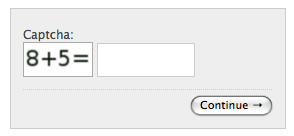
\includegraphics[width=.7\linewidth]{Images/StateOfArt/math_CAPTCHA}
         \caption{\footnotesize{With plain text.}}
     \end{subfigure}
     \hfill
     \begin{subfigure}[b]{0.48\textwidth}
         \centering
         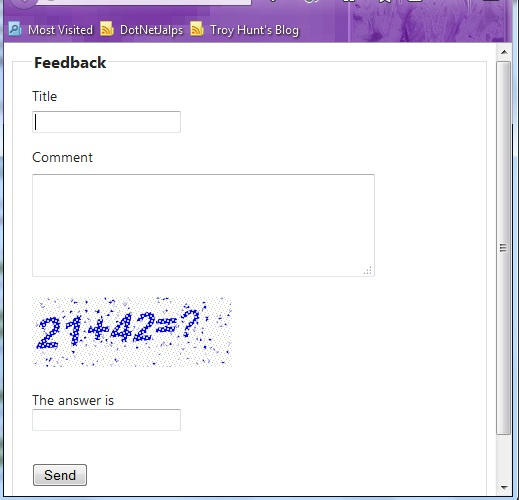
\includegraphics[width=.7\textwidth]{Images/StateOfArt/math_CAPTCHA2}
         \caption{\footnotesize{With wrapped text.}}
     \end{subfigure}
		\caption{\footnotesize{Example of arithmetic CAPTCHAs.}}
		\label{soa:arithmetic}
\end{figure}
An advanced version of this CAPTCHA is used in the Quantum Random Bit Generator Service (QRBGS) sign-up Web Page\cite{math_CAPTCHA} (see Figure \ref{soa:QRBGS}). This type of CAPTCHA asks user to solve an advanced math expression. It prevents the use of free or commercial OCRs because many mathematical symbols are not considered in their detection algorithm.\\
Hence many math symbols are wrongly translated by bot programs and the challenge is very secure. The only problem is that this CAPTCHA is very complex for normal users and many of them could not solve the challenge correctly.
\begin{figure}[h]
     \centering
     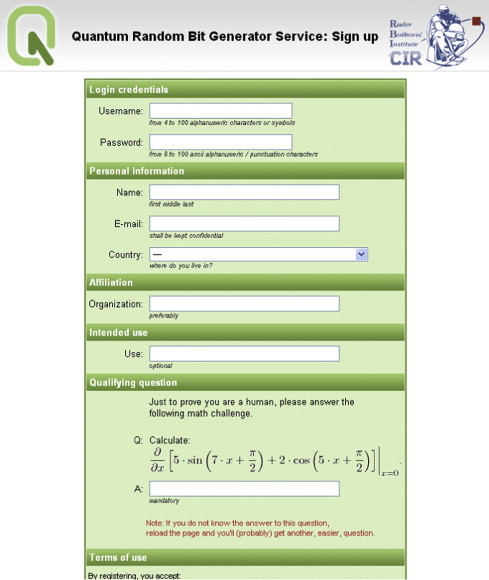
\includegraphics[width=.8\linewidth]{Images/StateOfArt/QRBGS}
     \caption{\footnotesize{Example of Quantum Random Bit Generator Service (QRBGS) sign-up Web Page \cite{math_CAPTCHA}.}}\label{soa:QRBGS}
\end{figure}
}
\vspace{3cm}
\item{\textbf{Audio-based}\\
this type of CAPTCHAs asks the user to type the words listened by an audio file (see Figure \ref{soa:audio_CAPTCHA}). It's developed for vision-impaired users. It usually has problems related to the language dictionary, from which words are taken, and the similarity of the sound between several words. This type of CAPTCHAs is vulnerable to many Automatic Speech Recognition (ASR) programs\cite{improving_audio}.
\vspace{2cm}
\begin{figure}[h]
     \centering
     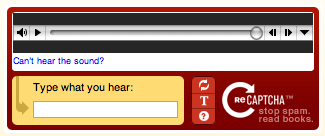
\includegraphics[width=.6\linewidth]{Images/StateOfArt/audio_CAPTCHA}
     \caption{\footnotesize{Example of audio-based CAPTCHA.}}\label{soa:audio_CAPTCHA}
\end{figure}
}
\item{\textbf{Game-based}\\
This type of CAPTCHAs performs the verification of the user nature through a set of several kind of games (see Figure \ref{soa:game}). This type of CAPTCHAs is called \textit{Dynamic Cognitive Game (DCG)} is usually developed using Flash and HTML5 with JavaScript. These technologies download the game code to the client and execute it locally. The only difficult for the bot to attack the challenge is the encryption/obfuscation of the code. This strategy prevent the store of the code onto different internet domains. However for example, there exists a bot attack, called \textit{Stream Relay Attack}, that obtains good results bypassing these challenges \cite{game_CAPTCHA}.
\begin{figure}[h]
     \centering
     \begin{subfigure}[b]{0.48\textwidth}
         \centering
         
\includegraphics[width=.9\linewidth]{Images/StateOfArt/game_CAPTCHA}
     \end{subfigure}
     \hfill
     \begin{subfigure}[b]{0.48\textwidth}
         \centering
         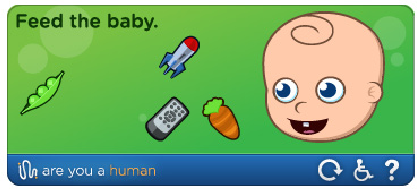
\includegraphics[width=.9\linewidth]{Images/StateOfArt/game_CAPTCHA2}
     \end{subfigure}
		
	 \begin{subfigure}[b]{0.55\textwidth}
         \centering
         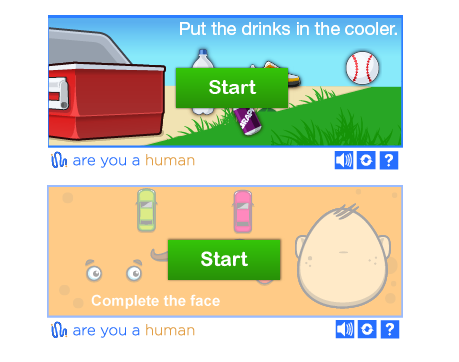
\includegraphics[width=\linewidth]{Images/StateOfArt/game_CAPTCHA3}
     \end{subfigure}
     \caption{\footnotesize{Examples of game-based CAPTCHAs.}}
     \label{soa:game}
\end{figure}
}
\item{\textbf{Image-based}\\
this type of CAPTCHAs asks to select the images that contain a requested subject. The set of images, on which the user needs to identify the subject, can be implemented in different ways, for example:
\begin{itemize}
\item{An image is divided into a set of sub-squares and each of them is a candidate image\ref{soa:image}}
\item{There are many images, each one with a unique different subject (see Figure \ref{soa:image2})}
\end{itemize}
This type of CAPTCHAs is vulnerable to different Computer Vision techniques Object Recogni
An extension of this type of CAPTCHAs, called \textit{FaceDCAPTCHA}, has been introduced\cite{FaceDCAPCTHA}. It incorporates elements of face detection. The human brain is very effective in the process of natural face segmentation even if there are complex backgrounds. This approach increases the security efficiency because the Computer Vision programs can easily detect if there is a face, e.g. Viola-Jones algorithm\cite{Viola_Jones}, but have many problems differentiating real and non-real photographs of faces.
\begin{figure}[h]
     \centering
     \begin{subfigure}[b]{0.48\textwidth}
         \centering
         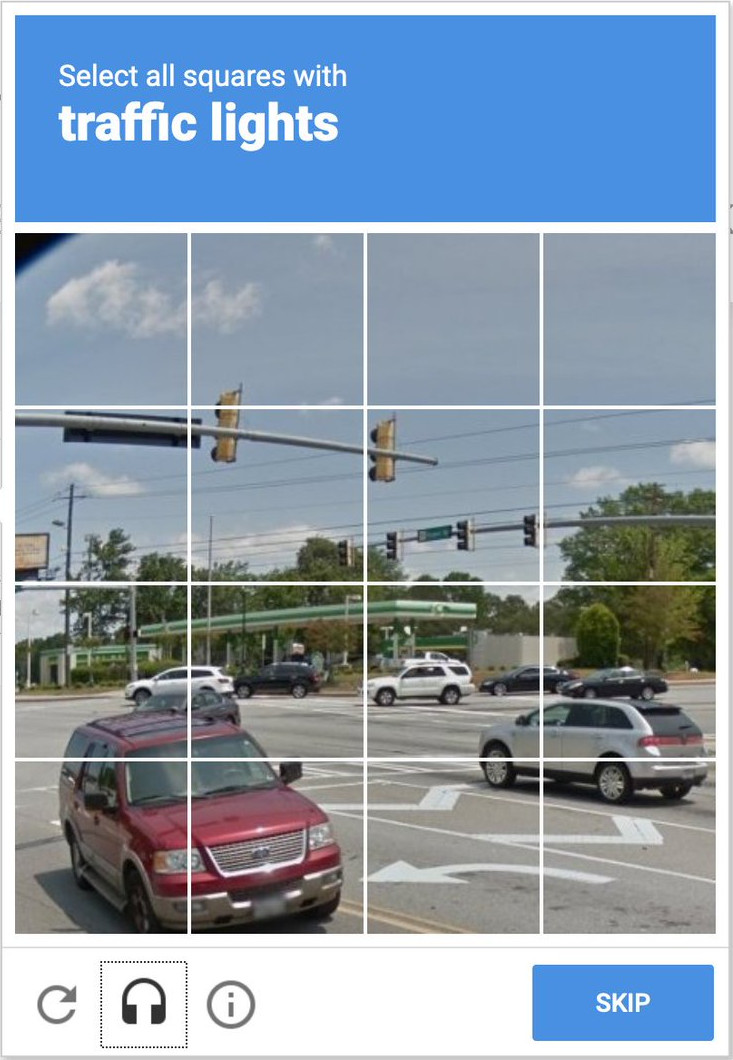
\includegraphics[width=.9\linewidth]{Images/StateOfArt/image_CAPTCHA}
         \caption{\footnotesize{With an image divided in sub-squares.}}
         \label{soa:image}
     \end{subfigure}
     \hfill
     \begin{subfigure}[b]{0.48\textwidth}
         \centering
         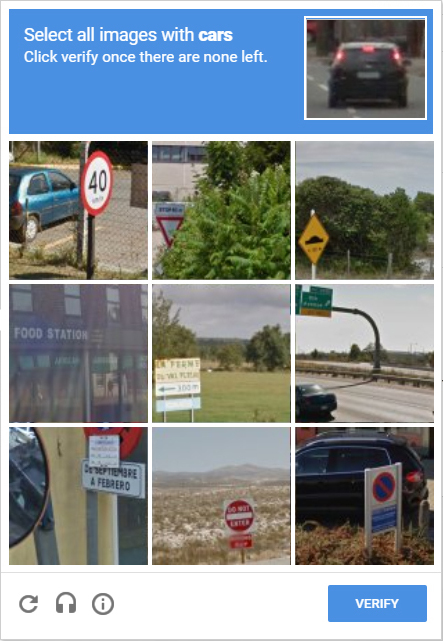
\includegraphics[width=.9\linewidth]{Images/StateOfArt/image_CAPTCHA2}
         \caption{\footnotesize{With several images.}}
        \label{soa:image2}
     \end{subfigure}
     \caption{\footnotesize{Examples of image-based CAPTCHAs.}}
\end{figure}
}
\item{\textbf{Puzzle-based}\\
this type of CAPTCHAs asks the user to complete a visual puzzle, created by dividing a given image in a set of pieces\cite{survey_CAPTCHA} (see Figure \ref{soa:puzzle}).\\
The task isn't easy for users because this type of CAPTCHAs takes more time to solve the puzzle but the security level is very high\cite{survey_CAPTCHA}. To improve the usability of the CAPTCHA, there exists a variant of the puzzle-based CAPTCHA in which needs to insert only some pieces of the puzzle instead of completing the whole puzzle (see Figure \ref{soa:puzzle2}).
\begin{figure}[h]
     \centering
     \begin{subfigure}[b]{0.48\textwidth}
         \centering
         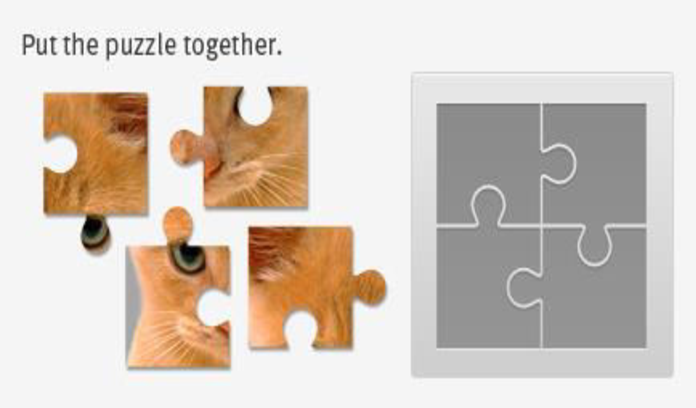
\includegraphics[width=.8\linewidth]{Images/StateOfArt/puzzle_CAPTCHA}
         \caption{\footnotesize{Completing the puzzle.}}
         \label{soa:puzzle}
     \end{subfigure}
     \hfill
     \begin{subfigure}[b]{0.48\textwidth}
         \centering
         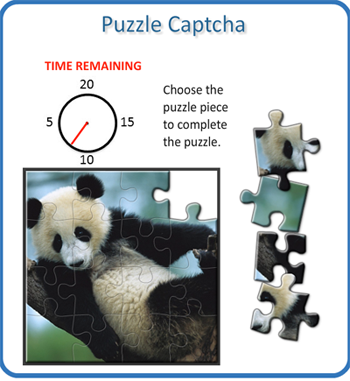
\includegraphics[width=.8\linewidth]{Images/StateOfArt/puzzle_CAPTCHA2}
         \caption{\footnotesize{Inserting only some pieces.}}
        \label{soa:puzzle2}
     \end{subfigure}
     \caption{\footnotesize{Examples of puzzle-based CAPTCHAs.}}
\end{figure}
}
\item{\textbf{Text-based}\\
this type of CAPTCHAs shows a series of wrapped characters and/or numbers on the screen. The users needs to understand which are the characters that composes the shown sequence and then type them inside a text-field. This type of CAPTCHAs is vulnerable to several type of attacks, related to Computer Vision techniques, that are:
\begin{itemize}
\item{OCR techniques\cite{OCR}}
\item{Segmentation techniques (e.g. DECAPTCHA\cite{DECAPTCHA})}
\item{Machine Learning and Deep Learning techniques}
\end{itemize}
In the design phase of a text-based CAPTCHA there are many issues, related to Computer Vision techniques, to be considered. For each of them, there is usually a solution in the design phase of the CAPTCHA that reduces the possibility that the challenge would be broken by a bot\cite{DECAPTCHA}.
\begin{figure}[h]
     \centering
     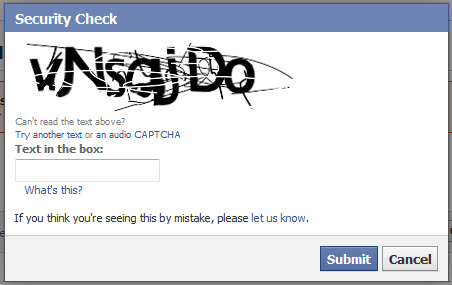
\includegraphics[width=.55\linewidth]{Images/StateOfArt/text_CAPTCHA}
     \caption{\footnotesize{Example of text-based CAPTCHA.}}\label{soa:audio_CAPTCHA}
\end{figure}
}
\item{\textbf{Video-based}\\
this type of CAPTCHA is not very common because of the weight of the file to be downloaded\cite{survey_advanced_CAPTCHA}. The traditional video-based CAPTCHA is composed by a video in which a sliding text is shown (see Figure \ref{soa:video}). The user needs to type this message in a text field to pass the challenge. Some implementations of this type of CAPTCHAs are vulnerable to machine learning attacks.\\
Another similar and interesting variant of this CAPTCHA is the \textit{Motion CAPTCHA}\cite{Motion_CAPTCHA}, developed by M. Shirali-shahreza and S. Shirali-shahreza, in which the user needs to watch a video. Then he needs to select which action was performed in the played file, choosing it from multiple answers (see Figure \ref{soa:video2}). The strength of these implementations of CAPTCHAs depends on the relationship between the multiple choices submitted to the user\cite{video_attack}.
\begin{figure}[h]
     \centering
     \begin{subfigure}[b]{0.48\textwidth}
         \centering
         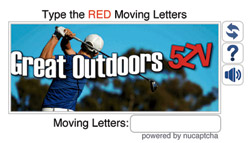
\includegraphics[width=\linewidth]{Images/StateOfArt/video_CAPTCHA}
         \caption{\footnotesize{Example of sliding text in video.}}
         \label{soa:video}
     \end{subfigure}
     \hfill
     \begin{subfigure}[b]{0.48\textwidth}
         \centering
         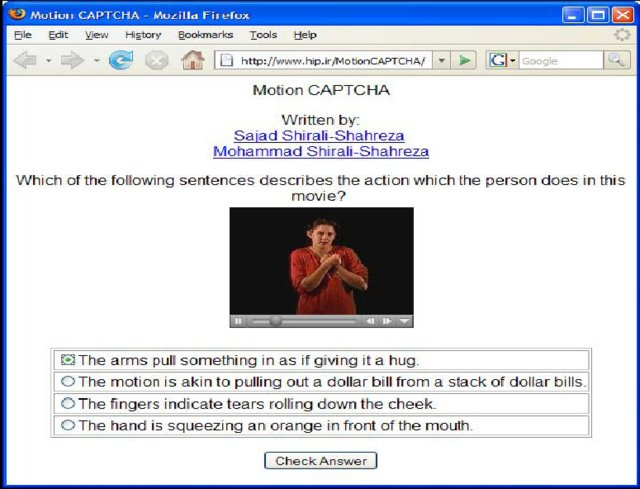
\includegraphics[width=\linewidth]{Images/StateOfArt/video_CAPTCHA2}
         \caption{\footnotesize{Example of Motion CAPTCHA\cite{Motion_CAPTCHA}.}}
        \label{soa:video2}
     \end{subfigure}
     \caption{\footnotesize{Examples of video-based CAPTCHAs.}}
\end{figure}
}
\end{itemize}
Some types of CAPTCHA don't destroy a session, after the correct answer is inserted by the user\cite{text_audio}. Hence, the hacker can crack following accesses using the same session id with the related solution of the challenge, after connecting to the web page of CAPTCHA. In this way the attacker can make hundreds of requests before the session expires and the previous operation must be computed again.\\
More details about the particular implementations of many of previously mentioned CAPCTHAs types are explained in the article of Walid Khalifa Abdullah Hasan\cite{survey_advanced_CAPTCHA}. With respect to user experience, the most enjoyable CAPTCHAs are usually the game-based and image-based ones but the most frustrating CAPTCHA is the text-based one\cite{usability_CAPTCHA}. A summary of usability and security issues is shown in Table \ref{soa:traditional_table}.

\section{Alternatives}
This types of CAPTCHA and authentication mechanisms are far from traditional CAPTCHAs and aren't based on cognitive knowledge of the human user but on other parameters:
\begin{itemize}
\item{\textbf{Biometrics-based}\\
}
\item{\textbf{Behavioural-based}\\
}
\item{\textbf{Social media sign-in}\\
}
\end{itemize}

\begin{sidewaystable}
\centering \footnotesize
\renewcommand*\arraystretch{1.3}
\begin{tabular}{cll}
\hline
\multicolumn{1}{c}{\textbf{CAPTCHA type}} & \multicolumn{1}{c}{\textbf{Usability issues}} & \multicolumn{1}{c}{\textbf{Security}}\\
\hline
\textit{Arithmetic (Math)} & {To be more effective, it requires advanced math knowledge.} & {Vulnerable to OCR techniques.}\\
\hline
\textit{Audio-based} & {
  \begin{minipage} [t] {0.4\textwidth}
  Issues of recognition:\\
      \begin{tabitem}
        \item{Previous knowledge of English dictionary by the user.}
        \item{Some character sounds very similar to others.}
      \end{tabitem} 
  \end{minipage}
} & {
  \begin{minipage} [t] {0.4\textwidth}
  It's vulnerable to ASR programs.
  \end{minipage}
}\\
\tabularnewline
\hline
\textit{Game-based} & {No problem} & {Vulnerable to Stream Relay Attack}\\
\hline
\textit{Image-based} & {
 \begin{minipage} [t] {0.4\textwidth}
Difficulty of identification of images caused by:\\
      \begin{tabitem}
        \item{Blur of images.}
        \item{Low vision condition.}
       \end{tabitem} 
  \end{minipage}
} & {}\\
\tabularnewline
\hline
\textit{Puzzle-based} & {Too much time to solve the puzzle} & {No significant issues}\\
\hline
\textit{Text-based} & 
{
  \begin{minipage} [t] {0.4\textwidth}
	Many problems have to be solved by user:\\
      \begin{tabitem}
        \item{Multiple fonts.}
        \item{Font size.}
        \item{Blurred Letters}
        \item{Wave Motion.}
       \end{tabitem} 
  \end{minipage}
} & 
{
  \begin{minipage} [t] {0.4\textwidth}
	It can be identified by:\\
      \begin{tabitem}
        \item{OCR technique}
        \item{Segmentation techniques}
        \item{Machine Learning and Deep Learning techniques}
       \end{tabitem} 
  \end{minipage}
}\\
\tabularnewline
\hline
\textit{Video-based} & {Heavy file to be downloaded} & {}\\
\hline
\end{tabular}
\caption{\footnotesize{Survey of main types of traditional CAPTCHAs\cite{survey_CAPTCHA}.}}
\label{soa:traditional_table}
\end{sidewaystable}

\begin{sidewaystable}
\centering \footnotesize
\renewcommand*\arraystretch{1.3}
\begin{tabular}{ccll}
\hline
\multicolumn{1}{c}{\textbf{Alternative Type}} & \multicolumn{1}{c}{\textbf{Name of implementation}} & \multicolumn{1}{c}{\textbf{Usability issues}} & \multicolumn{1}{c}{\textbf{Security}}\\
\hline
\textit{} & {} & {}\\
\hline
\end{tabular}
\caption{\footnotesize{Survey of main types of alternatives of CAPTCHAs\cite{survey_CAPTCHA}.}}
\label{soa:traditional_table}
\end{sidewaystable}